%!TEX root = ../proyecto.tex
\chapter{Desarrollo de pruebas y análisis de resultados.}
\section{Entorno de pruebas.}
Para el desarrollo de las pruebas, mi ordenador personal ha sido utilizado. Las especificaciones ténicas relevantes del mismo son:

\begin{itemize}
\item \textbf{GPU}: \underline{Zotac GeForce GTX 1060 AMP! Edition.}
\end{itemize}

% Please add the following required packages to your document preamble:
% \usepackage{booktabs}
% \usepackage{longtable}
% Note: It may be necessary to compile the document several times to get a multi-page table to line up properly
\begin{longtable}{@{}lc@{}}
\toprule
\multicolumn{1}{c}{\textbf{Características}}     & \textbf{Valor}           \\* \midrule
\endfirsthead
%
\endhead
%
\bottomrule
\endfoot
%
\endlastfoot
%
\textbf{Núcleos CUDA}                            & 1290                     \\
\textbf{Frecuencia del procesador}               & 1771 MHz                 \\
\textbf{Frecuencia de la memoria}                & 4004 Mhz                 \\
\textbf{Memoria global total}                    & 6 GB DDR5                \\
\textbf{Bus de memoria}                          & 192-bit                  \\
\textbf{Compute Capability}                      & 6.1                      \\
\textbf{Número de hebras por bloque}             & 1024                     \\
\textbf{Dimensión máxima del bloque (x, y, z)}   & 1024, 1024, 64           \\
\textbf{Dimensión máxima del ``grid'' (x, y, z)} & 2147483647, 65535, 65535 \\
\textbf{Número de registros por bloque}          & 65536                    \\
\textbf{Memoria compartida por bloque}           & 49152 KB                 \\
\textbf{Número de multiprocesadores}             & 10                       \\
\textbf{Modelo de driver CUDA}                   & WDDM                     \\
\textbf{Versión del driver CUDA}                 & 417.35                   \\
\textbf{Versión del SDK CUDA}                    & 10.0                     \\* \bottomrule
\caption{Características de la GPU NVIDIA GeForce GTX 1060 6 GB}
\label{tab:esptec}\\
\end{longtable}

\begin{itemize}
	\item \textbf{Placa Base:} MSI B450M Bazooka.
	\item \textbf{Sistema Operativo:} Windows 10 Home 64 bits.
	\item \textbf{CPU:} AMD Ryzen 5 2600X.
	\item \textbf{RAM:} Kingston HyperX Fury Black DDR4 2400 MHz PC4-19200 8GB CL15.
\end{itemize}
\section{Conjuntos de datos utilizados.}

Durante la fase de desarrollo del mapa auto-organizado hemos utilizado el conjunto de datos de las \textbf{caras de Olivetti}, creado por \textit{AT\&T Laboratories Cambridge} y descargada a través del paquete de Python \textit{scikit-learn} \cite{olivetti}. Dicho conjunto de imágenes consiste en 400 imágenes de 40 sujetos en escala de grises. Cada muestra son los valores de intensidad de cada píxel con un valor normalizado entre 0 y 1. Además, se proporciona una etiqueta que indica a qué sujeto pertenece cada imagen, pero para los propósitos de nuestro modelo de aprendizaje no supervisado la misma no será utilizada. Las imágenes están en una versión cuadrada de 64x64 píxeles dándonos un total de 4096 valores de intensidad por muestra. \\


Para evaluar el rendimiento de ambos modelos para conjuntos de \textit{Big Data} hemos utilizado \textbf{SUSY} \cite{susy}. Este conjunto de datos contiene 5 millones de muestras con 18 atributos, que se generó a partir de un experimento de física en el que también se intenta diferenciar un proceso que genera partículas supersimétricas (\textit{signal}) de otro proceso que no las genera (\textit{background}). En el caso del mapa auto-organizado, la clase de salida es ignorada. De manera similar al anterior, los datos del conjunto fueron generados a partir de simulaciones de Monte Carlo.


\section{Experimentos para evaluar el mapa auto-organizado.}
\subsection{Verificación de la implementación del modelo.}
En el caso del mapa auto-organizado, tanto la versión como para CPU como para GPU ejecutan el mismo algoritmo, por lo que las métricas de interés durante las ejecuciones realizadas son el tiempo de ejecución y la ganancia. En primer lugar, durante la fase de desarrollo usamos el conjunto de las caras de \textit{Olivetti}, que nos permitió comprobar de manera empírica y visual que los resultados obtenidos por el algoritmo son son correctos. En caso de funcionar correctamente, obtendríamos un conjunto de imagenes con la misma dimensión del mapa de neuronas, que son o se parecen a algunas de las caras de los sujetos, y donde las imágenes más parecidas se encuentran próximas las unas con las otras. \\

Para este experimento generamos un mapa de 5 filas y 6 columnas y ejecutamos el algoritmo durante 50 iteraciones, con 25 para la primera fase y otras 25 para la segunda fase y con los parámetros de control $\sigma_0, \sigma_f$ y $\tau$ a 3, 0,1 y 50, respectivamente. El \textit{RDD} de Spark que contiene las muestras de entrada es configurado para utilizar 10 particiones. Mientras que las versiones para CPU y GPU hacen exactamente lo mismo, utilizan métodos distintos para la generación de los pesos aleatorios iniciales. Por ello, para este experimento de verificación, tomamos también las dos medidas de calidad del mapa auto-organizado consideradas: el error de cuantificación y el error topográfico.\\

\begin{figure}[ht]
\centering
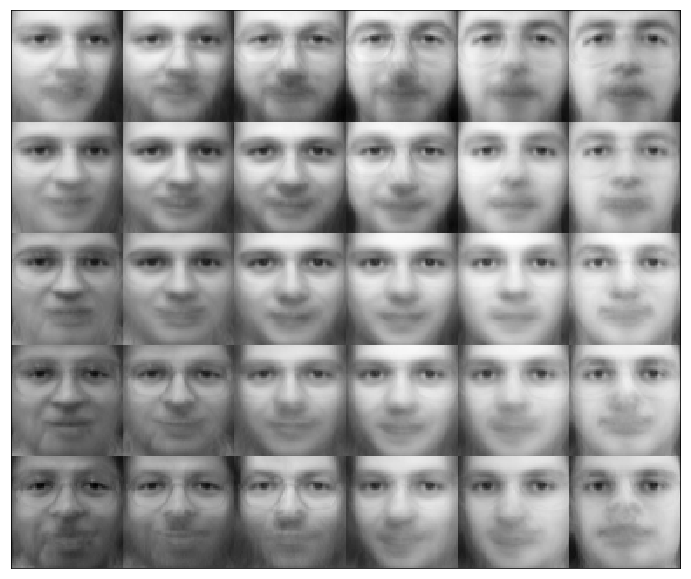
\includegraphics[scale=0.3]{imagenes/facescpu.png}
\caption{Imagen obtenida en el experimento para CPU del mapa auto-organizado.}
\label{img:somcpu}
\end{figure}

\begin{figure}[ht]
\centering
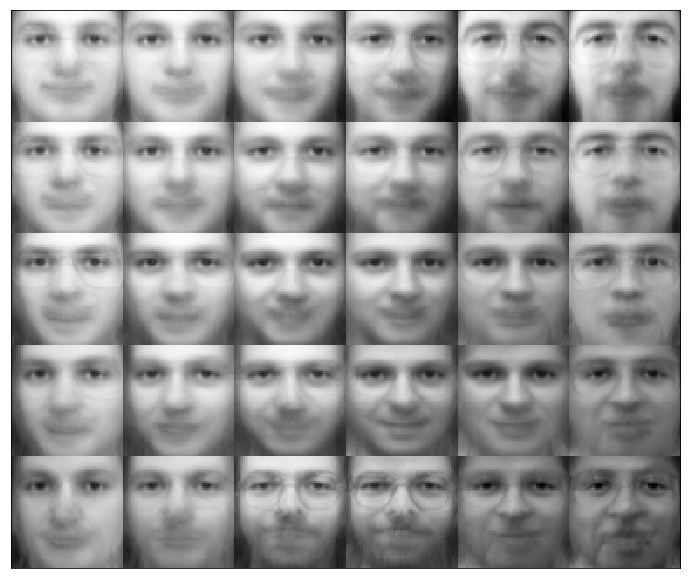
\includegraphics[scale=0.3]{imagenes/facesgpu.png}
\caption{Imagen obtenida en el experimento para GPU del mapa auto-organizado.}
\label{img:somgpu}
\end{figure}

En la figura \ref{img:somcpu}, podemos observar los resultados obtenidos para la ejecución de este algoritmo sobre CPU. En ella, podemos observar que, personas con piel de color más oscuro se agrupan en la esquina superior izquierda, o que, en la fila inferior nos encontramos ante imágenes de la misma persona, donde en las 2 primeras imágenes el sujeto está mirando de lado y, en las siguientes, parece llevar gafas puestas, entre otros detalles. En este ejemplo obtenemos un error de cuantificación de 6,57 y un error topográfico de 0,0325, tardando un total de 203,09 segundos en su ejecución.\\

En la figura \ref{img:somgpu}, podemos observar los resultados obtenidos para la ejecución de este algoritmo sobre nuestro dispositivo \textit{CUDA}. En ella, podemos observar como, personas que están claramente sonriendo se encuentran en la parte derecha de la penúltima fila, o en la esquina superior derecha, encontramos imágenes del mismo sujeto con gafas puestas. Para este ejemplo obtenemos un error de cuantificación de 6,56 y un error topográfico de 0,0125, tardando un total de 281,01 segundos en su ejecución.\\
	
En este pequeño experimento hemos podido comprobar visualmente que ambas implementaciones funcionan correctamente y proporcionan resultados similares, excepto en el tiempo de ejecución, y gran parte de los errores de implementación fueron detectados gracias a este experimento. El hecho de que la versión para GPU tarde más que la versión para CPU a que en cada una de las 10 particiones del \textit{RDD} se evalúan tan sólo 40 muestras y, nuestro algoritmo, en cada iteración y para cada partición, ha de realizar transferencias de memoria entre host y dipositivo, añadiendo un \textit{overhead}. Dado este número bajo de muestras, estamos invirtiendo más tiempo en realizar esas transferencias y lanzar los \textit{kernels} que en los pocos cálculos necesarios. Conforme el número de muestras sea mayor, como veremos en el siguiente experimento, iremos obteniendo mejores resultados con la GPU. 

\subsection{Uso del modelo sobre un conjunto de datos grandes dimensiones.}
Posteriormente, para evaluar la capacidad del algoritmo ante un conjunto de mayores dimensiones, utilizamos SUSY. Para este experimento ignoramos las etiquetas de salida y utilizamos un mapa de neuronas de 8 filas y 7 columnas con los parámetros de control $\tau$ a 10, $\sigma_0$ a 4, $\sigma_f$ a 0,1. El algoritmo lo ejecutamos durante 10 iteraciones (5 cada fase) y realizamos 4 repeticiones del experimento para tomar una medida de tiempo promedio, con el fin de obtener resultados más fiables que realizando una única ejecución. En este experimento nos centramos en evaluar como varía el tiempo de ejecución de nuestra implementación y la ganancia conseguida según vamos aumentando el número de muestras totales a evaluar. Para todos los experimentos nuestro RDD tendrá 10 particiones e iremos variando la cantidad de muestras totales de SUSY que vamos a procesar.

\begin{table}[ht]
\begin{tabular}{@{}l|c|c|c@{}}
\textit{\textbf{Nº de Muestras}} & \multicolumn{1}{l|}{\textit{\textbf{Tiempo CPU (s)}}} & \multicolumn{1}{l|}{\textit{\textbf{Tiempo GPU (s)}}} & \multicolumn{1}{l}{\textit{\textbf{Ganancia}}} \\ \midrule
\textit{\textbf{500000}}         & 231,09                                                & 56,99                                               & 4,06                                          \\
\textit{\textbf{1000000}}        & 426,19                                                & 58,74                                               & 7,26                                           \\
\textit{\textbf{1500000}}        & 618,29                                                & 61,41                                               & 10,07                                           \\
\textit{\textbf{2000000}}        & 822,55                                                & 62,73                                               & 13,11                                           \\
\textit{\textbf{2500000}}        & 1017,45                                               & 66,22                                               & 15,36                                           \\
\textit{\textbf{3000000}}        & 1212,12                                               & 67,75                                               & 17,89                                           \\
\textit{\textbf{3500000}}        & 1398,09                                               & 67,14                                               & 20,83                                           \\
\textit{\textbf{4000000}}        & 1616,68                                               & 67,63                                               & 23,90                                           \\
\textit{\textbf{4500000}}        & 1788,50                                               & 68,45                                               & 26,13                                           \\
\textit{\textbf{5000000}}        & 1992,61                                               & 72,30                                               & 26,99                                          
\end{tabular}
\caption{Tiempos promedios de ejecución y ganancias para el experimento del mapa auto-organizado sobre SUSY.}
\label{tab:susysom}
\end{table}

En la tabla \ref{tab:susysom} vemos las diferencias entre los tiempos promedios de 4 ejecuciones para CPU y 4 ejecuciones para GPU según los percentiles de muestras propuestos para el experimento. La evolución de los tiempos de ejecución para la GPU oscila en un pequeño intervalo entre los 60-70 segundos (1 minuto). Sin embargo, la evolución de los tiempos para la CPU oscila entre los 231 segundos (casi 4 minutos) y 1992 segundos (33 minutos) por ejecución.  Para una mejor visualización de estos resultados planteamos la gráfica de la figura \ref{img:somsusy}, en la que combinamos las gráficas de líneas para la evolución de los tiempos promedios con las ganancias obtenidas en una gráfico de barras. \\

\begin{figure}[ht]
\centering
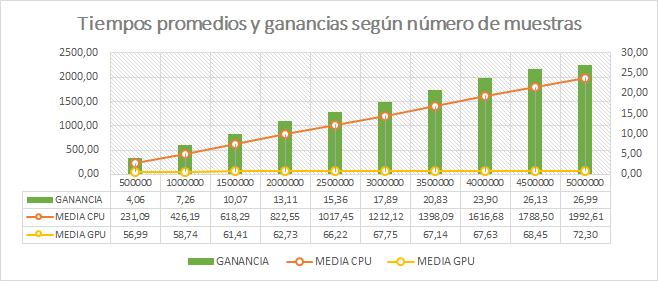
\includegraphics[scale=0.7]{imagenes/susysom.png}
\caption{Gráfica con tiempos promedios y ganancias para SUSY.}
\label{img:somsusy}
\end{figure}

En la gráfica planteada vemos de manera clara cómo, al aumentar el número de muestras, la implementación basada en \textit{CUDA} y \textit{Spark} es considerablemente más rápida que su homóloga para CPU. En el ejemplo más pequeño planteando, es decir, evaluar medio millón de muestras, en el que cada una de las 10 particiones del \textit{RDD} evalúa 50000 muestras, la versión para CUDA es 4 veces más rápida que su homóloga para CPU. En el ejemplo más grande propuesto, es decir, evaluar 5 millones de muestras, el uso de CUDA nos ofrece un tiempo de ejecución casi 27 veces más rápido que la CPU.


\subsection{Resultados de Nsight sobre la versión final del algoritmo.}
Por último, analizamos en profundidad simulamos el entrenamiento del SOM durante una iteración con un ejemplo completamente aleatorio. El total de muestras a evaluar es de 1 millón, divididas en 10 particiones de 100000 muestras. El mapa de neuronas objetivo es de 10 filas por 10 columnas y la dimensión del problema a resolver es de 18 características. En la tabla \ref{tab:profsomkernels}, vemos los tiempos de ejecución de los \textit{kernels} en este experimento.\\

\begin{table}[ht]
\begin{tabular}{@{}|lc|cccc|@{}}
\toprule
                                 & \multicolumn{1}{l|}{}                               & \multicolumn{4}{c|}{\textit{\textbf{Tiempo}}}                                                                                         \\
\textit{\textbf{Kernel}}         & \multicolumn{1}{l|}{\textit{\textbf{Nº usos}}} & \textit{\textbf{mínimo}} & \textit{\textbf{medio}}           & \textit{\textbf{máximo}}          & \textit{\textbf{total}}            \\ \midrule
\textit{\textbf{rand\_weights}}  & 1                                                   & $6,62 \; \mu s$             & $6,62 \; \mu s$                      & $6,62 \;\mu s$                      & $6,62 \;\mu s$                       \\
\textit{\textbf{som\_iter}}      & 10                                                  & $1,61 \; ms$                & $1,835 \; ms$                        & $2,17 \;ms$                         & $18,35 \;ms$                         \\
\textit{\textbf{finish\_update}} & 1                                                   & $37,38 \; \mu s$            & \multicolumn{1}{l}{$37,38\; \mu s$} & \multicolumn{1}{l}{$37,38 \;\mu s$} & \multicolumn{1}{l|}{$37,38 \;\mu s$} \\ \bottomrule
\end{tabular}
\caption{Tiempos de ejecución de los kernels en el experimento de profiling}
\label{tab:profsomkernels}
\end{table}

Como cabía esperar, la mayor parte del tiempo se corresponde a la ejecución del \textit{kernel som\_iter}, que tarda un total de $18,35 \; ms$. El kernel \textit{rand\_weigths} es el más rápido de todos y, aun así, es sólo invocado una vez en el algoritmo, independientemente del número de iteraciones, por lo que no tiene sentido centrarse en optimizarlo mientras se puedan hacer otras mejoras. El kernel \textit{finish\_update}, que será llamado tantas veces como iteraciones se realicen en el algoritmo ocupan el puesto intermedio, siendo 49 veces más rápido que una llamada al \textit{kernel som\_iter}. Además, el \textit{kernel som\_iter}, siempre será llamado las mismas veces que \textit{finish\_update} multiplicado por el número de particiones del \textit{RDD} por lo que, a ser posible, hemos de centrarnos en mejorar este \textit{kernel}.\\

\begin{figure}[ht]
\centering
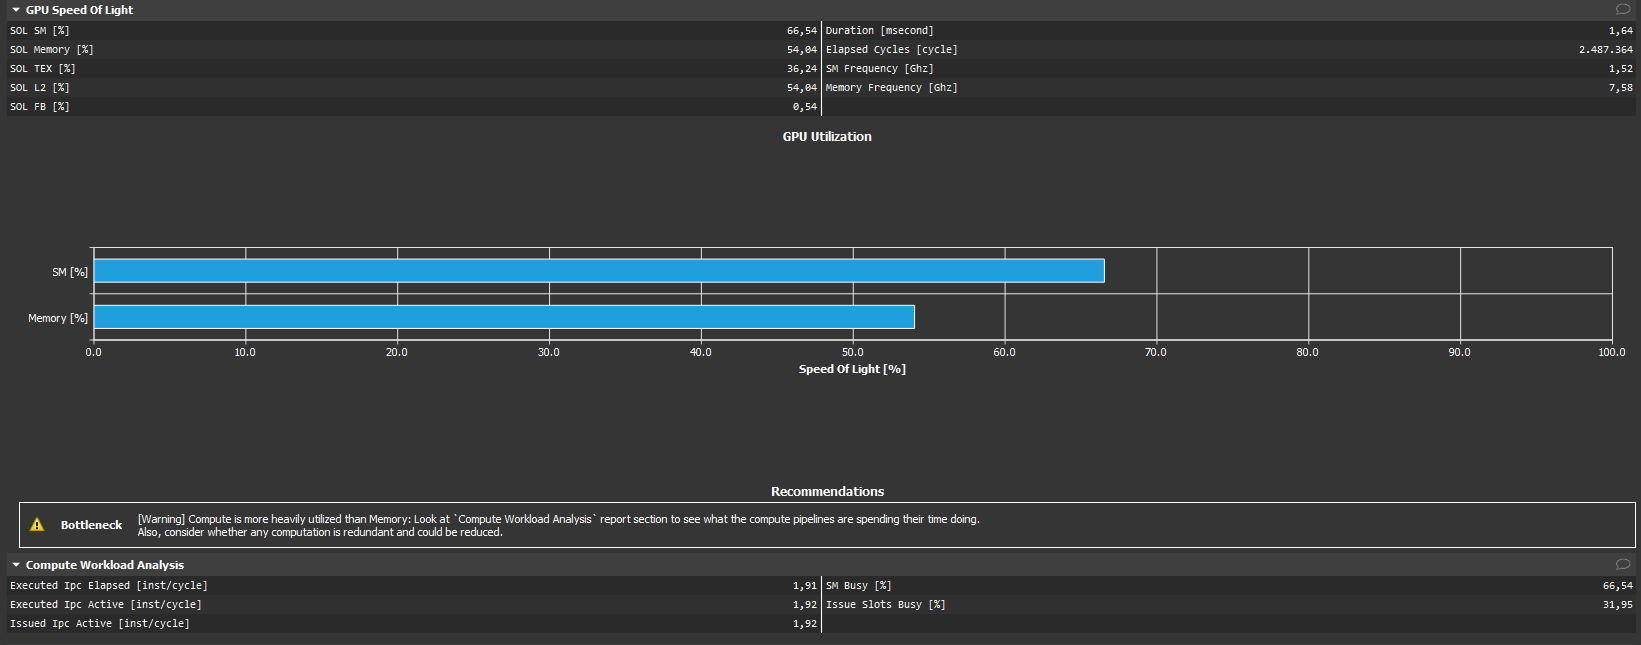
\includegraphics[scale=0.3]{imagenes/som_sol.png}
\caption{Speed of Light del kernel evaluado.}
\label{img:sol}
\end{figure}

Un análisis más profundo del \textit{kernel som\_iter} con el profiler nos revela que el cuello de botella se debe a los cálculos realizados (figura \ref{img:sol}). La medida \textit{``Speed Of Light (SOL)''} nos indica lo cerca que estamos de alcanzar el rendimiento teórico máximo de unidades de \textit{hardware} durante la utilización del dispositivo CUDA en el \textit{kernel}. Podemos observar que, en nuestro caso, estamos aprovechando un 66,54 \% de la capacidad máxima de computación de nuestra GTX 1060.\\

\begin{figure}[ht]
\centering
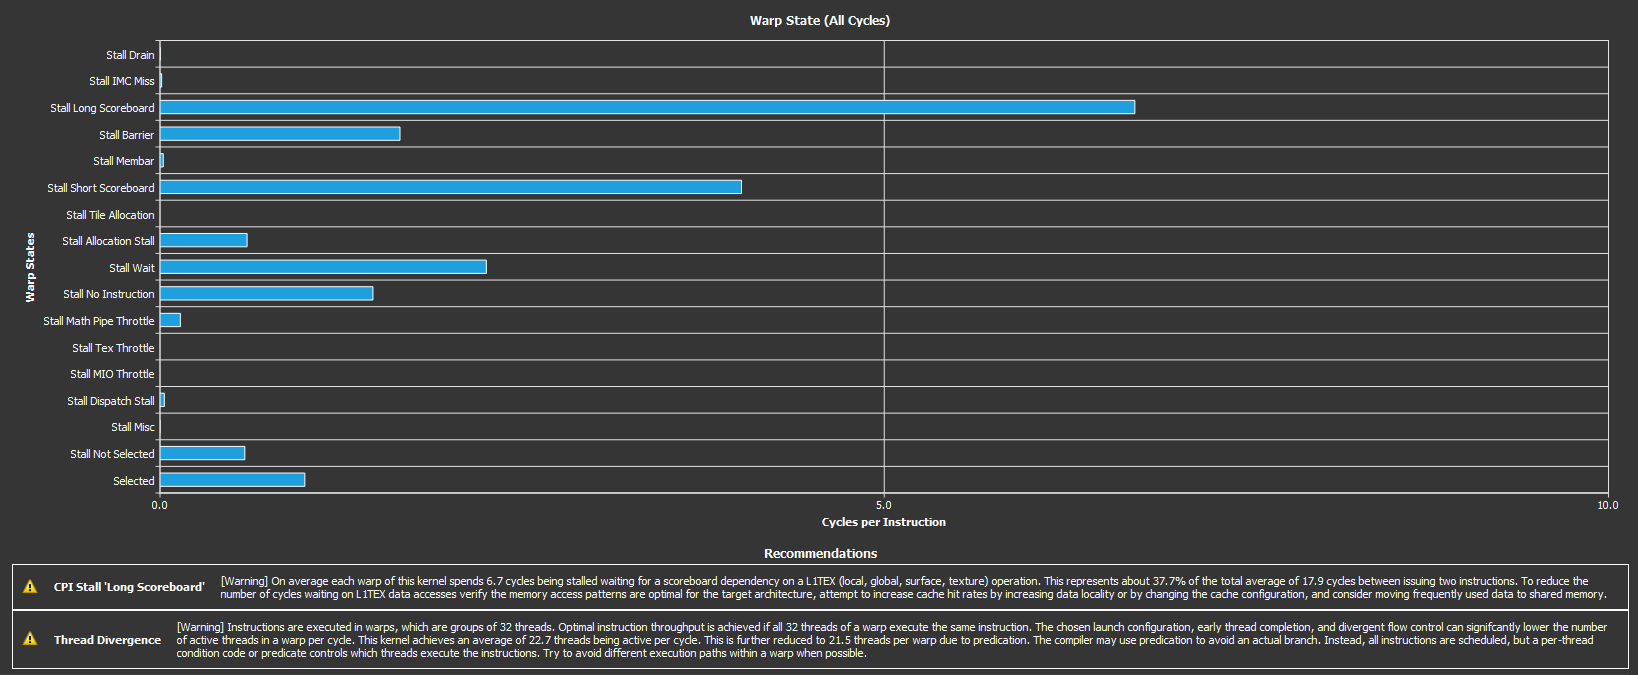
\includegraphics[scale=0.3]{imagenes/som_warp_states.png}
\caption{Análisis de los warps del kernel.}
\label{img:warpssom}
\end{figure}

En la figura \ref{img:warpssom} vemos las dos razones principales que hacen que el \textit{kernel} no funcione más rápido. Una de ellas es los accesos a memoria dentro del dispositivo y la otra es la divergencia de las hebras, es decir, situaciones en las que las hebras quieren ejecutar diferentes instrucciones.\\

 Todos los elementos dentro de un bloque que eran utilizados más de una vez fueron cargados en memoria compartida por lo que podemos intuir que este problema radica de conflictos que surjan del uso de las operaciones de suma atómica. Encontrar una alternativa mejor que la planteada para el cálculo de los pesos parciales debería de ser la prioridad a la hora de optimizar este algoritmo. \\

 Por otro lado, el segundo problema que destacamos es la divergencia, que se debe principalmente a que, en este ejemplo, trabajamos con 128 hebras por bloque mientras que el número de neuronas es 100, por lo que uno de los \textit{warps} utilizará tan sólo 4 de las 32 hebras. En un caso ideal, el tamaño del mapa tendría un número de neuronas que fuese potencia de 2 (al menos 32). Si tuviésemos garantizado que esto fuese a ocurrir, podríamos eliminar gran parte de los condicionales utilizados ya que no sería necesario comprobar si hay más hebras que neuronas, ni habría que rellenar distancias extras con infinito, ni tendríamos que realizar todas las comprobaciones en la reducción para tamaños de bloque superiores al número de neuronas.

\newpage